\documentclass[10pt]{article}
\usepackage[backend=bibtex,style=numeric]{biblatex}
\usepackage{enumitem}
\usepackage{graphicx}
\usepackage{caption}
\usepackage{subcaption}
\usepackage{fullpage}

\addbibresource{refs}

\title{Extracting Application and Menu Events from UI Tutorial Videos}
\author{Daniel Seita \& Andrew Head}

\begin{document}

\maketitle

\section{Introduction}

In this project, we present two main contributions. First, we show that a standard neural network
following the AlexNet architecture with minimal tweaking can accurately recognize frames belonging
to a class of videos.  Second, we present a pipeline and procedure for detecting menus within a
video frame sequence. We then discuss how these two stages might be combined to enhance the process
of extracting useful information from videos.

\subsection{Motivation}

The proliferation of video tutorials on using different software raises new research questions on
how to improve their use to help users learn software~\cite{matejka_ambient_2011,
pongnumkul_pause-and-play_2011}.  One strength of video tutorials may be that users can directly
observe expert use, which can serve as a strong learning aid. Grossman \& Fitzmaurice showed
benefits of brief contextual video clips: short, 10-25 second contextually available videos were
effective to help users accomplish task and retain what they learned than traditional text-based
tutorials~\cite{grossman_toolclips_2010}. Unfortunately, video tutorials have drawbacks. Navigation
issues could lead to misunderstanding of content, and users may not be able to keep up with the pace
of instruction. Researchers working with longer, 2-3 minute task-oriented tutorials found that users
performed better with text tutorials than videos because users could not work at the same pace as
the video~\cite{grabler_generating_2009}.

In general, research on instructional videos point shows a need to segmented videos to emphasize the
steps of the task. One way to do that might be to develop techniques for detecting locations of
certain menu actions in the video, such as when the video shows its user clicking on a button in a
Photoshop video to create a blank image. Our goal, therefore, is to utilize computer vision
techniques to aid in this process.


\subsection{Related Work}

By examining pixels, many have succeeded at reverse engineering user interfaces and interactions
with user interfaces with purely visual information, independent of any knowledge of underlying
application implementation. Work by Zettleymoyer et
al.~\cite{zettlemoyer_ibots_1999}~\cite{zettlemoyer_visual_1999} examine widget identification in
IBOTS and VisMap.  Also
see~\cite{potter_triggers_1992}~\cite{amant_image_2005}~\cite{lieberman_visual_2001}.  Visual
identification of widgets and UIs may also have also been used in Olsen et al.'s ScreenCrayons work
that links annotations to arbitrary screen elements~\cite{olsen_jr_implementing_1999}, and in Tan et
al.'s work to interactively subdivide windows with a copy-paste metaphor~\cite{tan_wincuts_2004}.
\textbf{Andrew: Check on this.}

More recently, Sikuli~\cite{yeh_sikuli_2009} uses computer vision to identify GUI elements from
screen captures, using template matching for small UI elements and voting based on invariant local
features for large elements.  In application, Sikuli allows users to search for documentation
related to screenshots taken of UI elements, and to script GUI tasks using visual cues of the UI.
For searching based on screenshots, 3 types of features are extracted: text from the source
document, visual words computed from visual words from MSER-detected salient elliptical patches, and
3-grams over widget-embedded text extracted through OCR.  For searching on the screen for saved
screenshot images, small patterns are found via template matching and large patterns through
invariant feature voting.

Pause-and-Play extends the template matching approach of Sikuli to detect tool-selection UI events
in compressed, low-resolution video tutorials.  The system takes a tool palette template and tool
icons as input, producing metadata file of tool changes with timecodes.  With template matching at
multiple resolutions, detection is invariant to recording resolution and some camera effects.  Their
system cannot be run in in real-time~\cite{pongnumkul_pause-and-play_2011}.

A number of different technologies attempt to learn templates for arbitrary UI
elements~\cite{chang_associating_2011}~\cite{dixon_prefab_2010}~\cite{hurst_automatically_2010}~\cite{matejka_ambient_2011}.
Learning may require access to mouse APIs~\cite{hurst_automatically_2010} and accessibility
APIs~\cite{chang_associating_2011}.

Prefab identifies GUI elements with GUI specific visual features~\cite{dixon_prefab_2010}, which
enables overlay of advanced interactions on existing
interfaces~\cite{dixon_content_2011}~\cite{dixon_general-purpose_2012}.  \textbf{Andrew: Check up on
this initial description.  I'm also not sure if Prefab actually belongs in this conceptual group.}
To delve into the technical implementations of the Prefab pixel-based matching algorithm, we report
from~\cite{dixon_general-purpose_2012}.  Prefab identifies interface elements using a library of
prototypes.  This uses two strategies: exact matches of prototype pixels against an image, and
modelining the prototype background and differencing pixel in an image to identify foreground
interface elements.  Prefab generalizes from example images to models which contain parts like exact
pixel features, or regions or areas of variable size or repeating patterns.  It organizes the entire
interface into a hierarchy.

Waken contributes to this space by discovering cursor shapes, clicking actions, icons, tooltips and
menus, all by examining the difference between frames of UI video.  They do this by making
assumptions about how the image of icons change during hover and press actions.  Detection of the
cursor and icons in later frames is performed by template matching~\cite{banovic_waken_2012}.  We
rely on techniques similar to those in Waken to establish when menus have been activated and menu
items selected.


\section{Video Classification}

This will be Daniel's section. I'm probably not going to include any subsections to save time.

Figure~\ref{fig:alex_net} shows our accuracy results for the two AlexNet networks we trained.

Figure~\ref{fig:per_class} shows our per-class accuracy results for the ``no noise'' AlexNet
network.

\begin{figure}[t]
\centering
  \begin{minipage}{.48\textwidth}
  \centering
  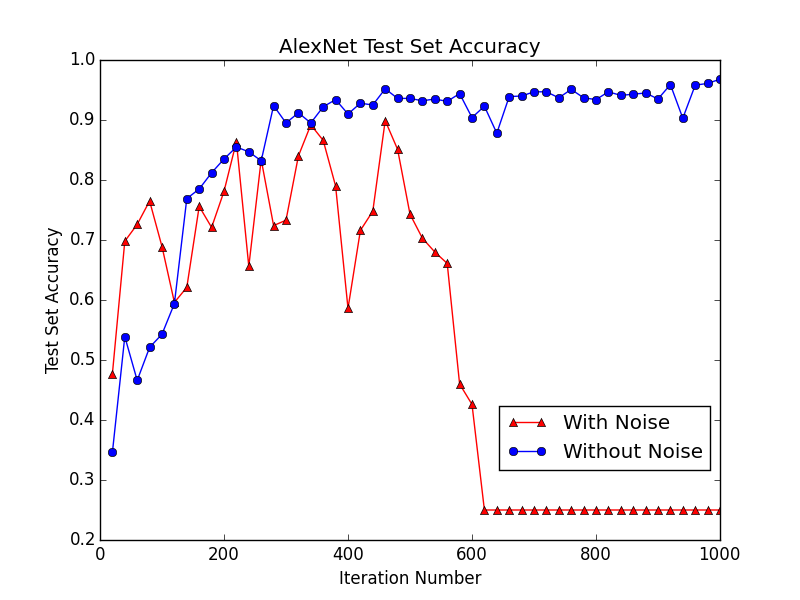
\includegraphics[width=1\linewidth]{AlexNet_Accuracy1000}
  \caption{AlexNet accuracy results of two networks trained on two image datasets.}
  \label{fig:alex_net}
  \end{minipage}\hfill
  \begin{minipage}{.48\textwidth}
  \centering
  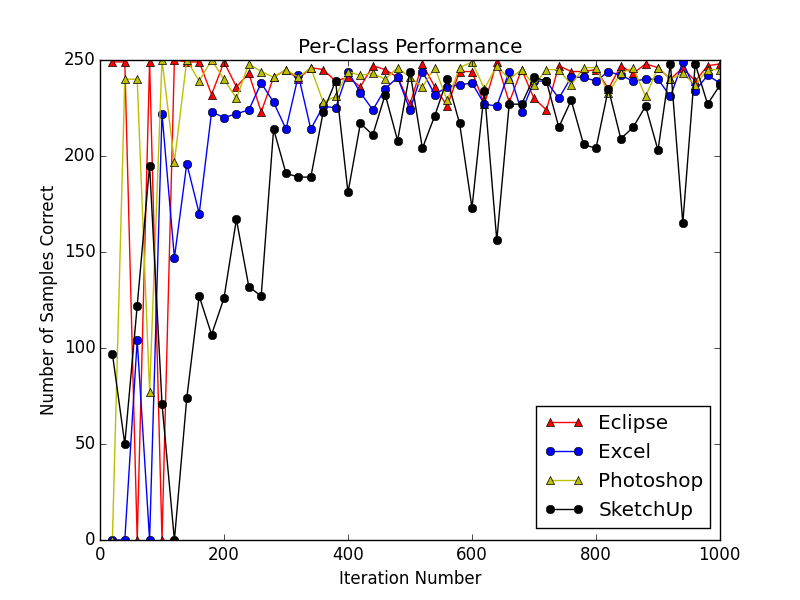
\includegraphics[width=1\linewidth]{PerClassPerformance1000}
  \caption{AlexNet per-class accuracy results for the network trained on ``no noise'' data.}
  \label{fig:per_class}
  \end{minipage}
\end{figure}

Figures~\ref{fig:filters_all} and~\ref{fig:filters_nonoise} show visualizations of the 96 filters in
the first layer of AlexNet, each of which has dimension $55\times 55$. These were taken for the
model that had 1000 iterations of training.

\begin{figure}[t]
\centering
  \begin{minipage}{.4\textwidth}
  \centering
  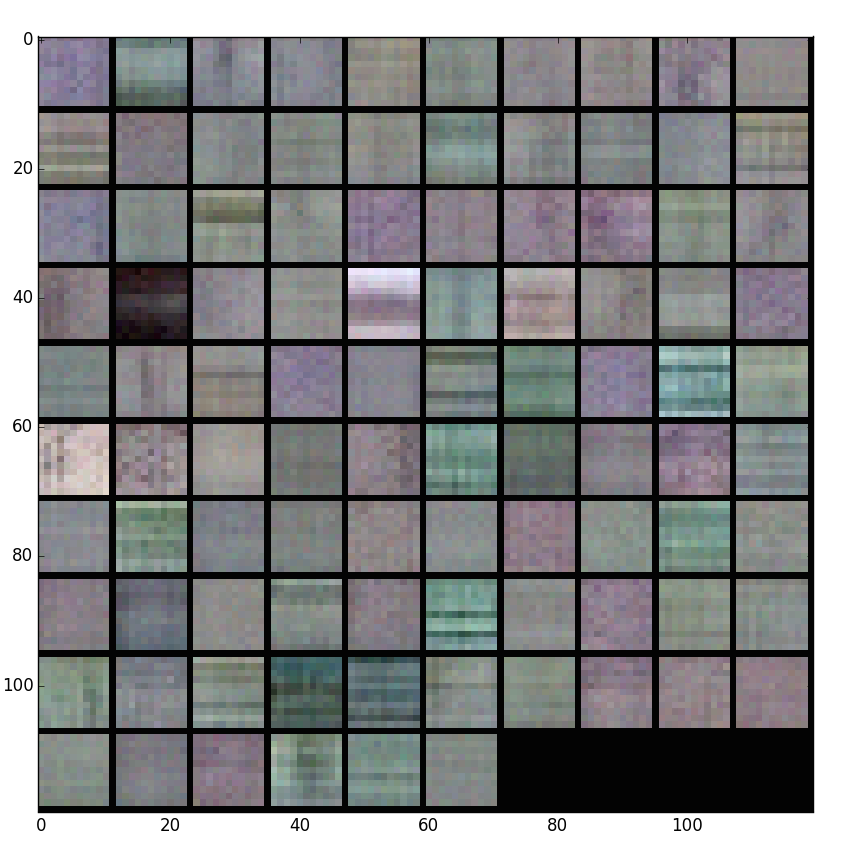
\includegraphics[width=1\linewidth]{Filters_All1000}
  \caption{Visualization of filters from the network trained on all our image data.}
  \label{fig:filters_all}
  \end{minipage}\hfill
  \begin{minipage}{.4\textwidth}
  \centering
  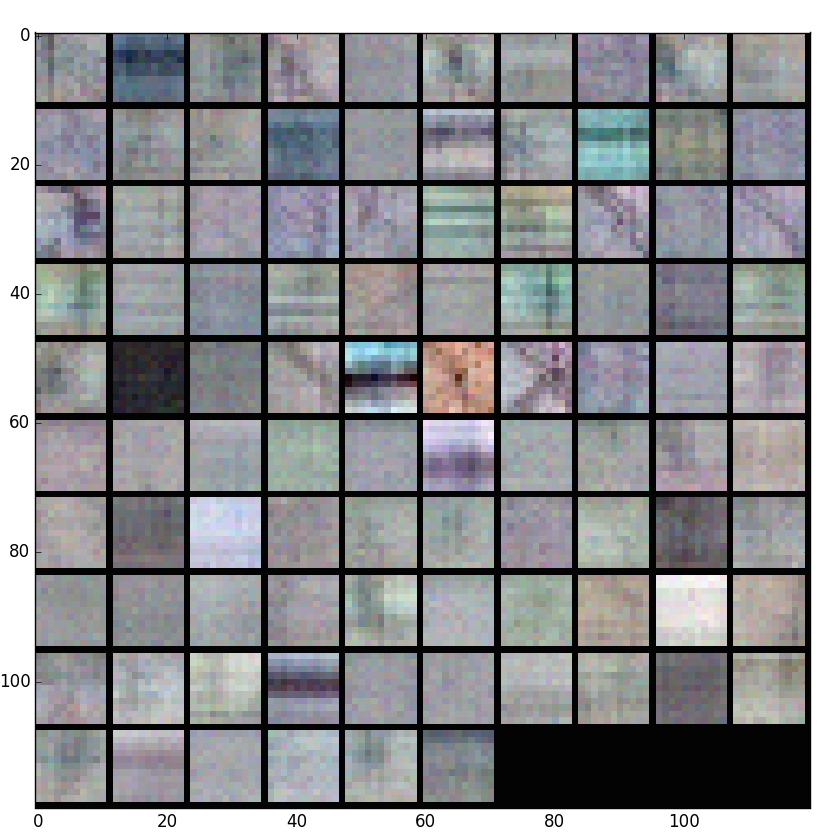
\includegraphics[width=1\linewidth]{Filters_NoNoise1000}
  \caption{Visualization of filters from the network trained on ``no noise'' image data.}
  \label{fig:filters_nonoise}
  \end{minipage}
\end{figure}

Finally, we performed a brief, informal experiment where we applied the neural network to videos that
were not part of our training or testing data. We chose one video for each of the four classes by
searching on Google Video ``X tutorial'' where ``X'' was replaced by one of the four video names.
The first video that was between 5 and 20 minutes long, and that was not already part of our
training/testing data, was selected. We extracted one frame per second for the four videos, and
deleted the first ten and final ten frames from consideration.

To classify the frames, we applied our AlexNet neural network trained on the ``noiseless'' data
after 1000 iterations. To describe the output, we use ``splits'' where $(a,b,c,d)$ indicates that
$a, b, c,$ and $d$ frames were classified as Eclipse, Excel, Photoshop, and SketchUp, respectively.
The splits were as follows: the Eclipse video had $(319,0,79,0)$, the Excel video had
$(610,0,71,7)$, the Photoshop had $(1,6,416,69)$, and the SketchUp had $(9,2,233,804)$. Clearly, for
the Eclipse, Photoshop, and SketchUp videos, the classifer was able to assign the vast majority of
frames to the correct class. If we were using this as part of an overall data mining pipeline, our
classifier would assign the video according to the most-assigned class, so three videos would be
classified correctly.

The Excel output is interesting, because our network thought most of the frames belonged to Eclipse
videos. A brief look at the video indicated that it had an introductory scene that took up ninety
seconds (and we only deleted the first 10 frames) and that it was about a newer version of Excel
(2013) than the ones that were trained in our network (2007). Still, it is unfortunate but shows
that we need to be able to provide a wider variety of training data.

\section{Locating Menus in a Frame Sequence}

This will be Andrew's section.

\subsection{Data}

Answer these questions:
\begin{enumerate}[noitemsep]
\item What is our dataset?
\item How did we construct/acquire it?
\item What's its size?
\item (optional) How will we improve it in the future?
\end{enumerate}


\subsection{Implementation}
Here's a figure of our (edit: Andrew's) pipeline.  \textbf{Andrew: Add figure of pipeline.}

\subsection{Menu Location Results}

Here we (edit: Andrew) want to touch upon:
\begin{enumerate}[noitemsep]
\item How reliably can we classify UI events?
\item How long does it take for us to process one minute of video?  What are
the practical implications of this?
\item Some images that show recognition results for a few representative
screenshots of user interfaces.
\end{enumerate}


\section{Discussion and Conclusion}

TODO (combining the two because we don't have a lot of space!)

We freakin' rock.

\printbibliography

\end{document}
